\chapter{Linear algebra}
\label{cha:linear_algebra} \defi{\textbf{Group} \label{def:group}\\In abstract algebra, a group is a set $G$ where an operation $*$ is defined. Moreover $*$ satisfies the following properties: \begin{enumerate}\item \textit{associative}: $(a*b)*c=a*(b*c) \forall a,b,c \in G$

\item \textit{identity element}: $\exists e \in G : a*e=e*a=a \forall a \in G$

\item \textit{inverse element}: $\forall a \in G$ $\exists a' \in G : a*a'=a'*a=e$\end{enumerate} }

\defi{\textbf{Commutative group} \label{def:comm_group}\\ A group $(G,*)$ is \textit{commutative} iff $a*b=b*a$ $\forall a,b \in G$. }

\defi{\textbf{Vector space} \label{def:vector_space}\\ A \textit{vector space} over the field $\mathcal{R}$ is an algebraic structure composed by a commutative group $(V,+)$, whose elements are called $vectors$, and a function $f:\mathcal{R}\times V \rightarrow V$ called \textit{scalar multiplication} which satisfies the properties listed below. It is common to use $kv$, instead of $f(k,v)$ to represent the scalar multiplication between a scalar $k \in \mathcal{R}$ and a vector $v \in V$. \begin{itemize}\item \textit{distributive over elements} $k(v_{1}+v_{2})=kv_{1}+kv_{2}$

\item \textit{distributive over scalars} $(k_{1}+k_{2})v=k_{1}v+k_{2}v$

\item \textit{associative over scalars} $(k_{1}k_{2})v=k_{1}(k_{2}v)$

\item \textit{identity element} $1v=v$\end{itemize} $\forall k,k_{1},k_{2}\in \mathcal{R}, \forall v, v_{1}, v_{2}\in V$. }
Vector space examples are: the set of two-dimensional vectors $V^{2}$, the set
of three-dimensional vectors $V^{3}$, the matrix space $M_{m,n}(\mathcal{R})$.

\defi{\textbf{Subspace} \label{def:subspace}\\ Given a vector space $V$ defined over the field $R$, a non-empty set $W \subseteq V$ is a \textit{subspace} of $V$ if it is close w.r.t. the sum of vectors and the scalar product: \begin{equation*}\forall w,w'\in W, \forall k \in K, w+w' \in W \wedge kw \in W\end{equation*} Each subspace is in turn a vector space with respect to the operations defined in $V$. }

\defi{\textbf{Linear combination} \label{def:linear_combination}\\ Given a vector $v \in V$, $v$ is a linear combination of the vectors $v_{1},...,v_{k}\in V$ with coefficients $c_{i}\in \mathcal{R}$ if: \begin{equation*}v = c_{1}v_{1}+...+c_{k}v_{k}= \sum_{i=1}^{K}c_{i}v_{i}\end{equation*} }

\defi{\textbf{Span} \label{def:span}\\ The span of vectors $v_{1},...,v_{k}$ is defined as the set of their linear combinations: \begin{equation*}\{\sum_{i=1}^{K}c_{i}v_{i}, c_{i}\in \mathcal{R}\} = <v_{1},...,v_{k}>\end{equation*} The span is a \textit{vector subspace} (also known as \textit{linear subspace}) of $V$. In particular the span $<v_{1},...,v_{k}>$ is the subset generated by $v_{1},...,v_{k}$. }

\defi{\textbf{Linear independency and linear dependency} \label{def:indipendency1}\\ A set of vectors $v_{1},...,v_{k}$ is \textit{linearly independent} if the null vector can be written as a linear combination of the elements $v_{i}$ of the set

\begin{equation*}a_{1}v_{1}+a_{2}v_{2}+...+a_{k}v_{k}=0\end{equation*}

if and only if all the coefficients $a_{1},...,a_{k}$ are null. Intuitively, a set of vectors $v_{1},...,v_{k}$ is linearly independent if none of them can be written as a linear combination of the others. \\ A set of vectors $v_{1},...,v_{k}$ is \textit{linearly dependent} is it is not linearly independent. As a consequence, a set of vectors $v_{1},...,v_{k}$ is linearly dependent if there exist some not-null scalars $a_{1},...,a_{k}$ such that: \begin{equation*}a_{1}v_{1}+a_{2}v_{2}+...+a_{k}v_{k}=0\end{equation*} }

\defi{\textbf{Basis} \label{def:basis1}\\ A set of vectors $\mathcal{B}=\{v_{1},...,v_{k}\}$ is a \textit{basis} for $V$ if any element in $V$ can be uniquely written as a linear combination of vectors $v_{i}$. A necessary condition is that vectors $v_{i}$ are linearly independent. All bases of $V$ have the same number of elements, called the \textit{dimension} of the vector space. }
\defi{\textbf{Linear maps} \label{def:linear_maps}\\ Given two vector spaces $V$ and $V'$, a function $f: V \rightarrow V'$ is a \textit{linear map} if $\forall a_{1}, a_{2}\in \mathcal{R}, v_{1}, v_{2}\in V$: \begin{equation*}f(a_{1}v_{1}+a_{2}v_{2})=a_{1}f(v_{1})+a_{2}f(v_{2})\end{equation*} }

A linear map between two finite-dimensional spaces $V$, $V'$ of dimensions $n$,$m$
can always be written as a matrix $A$. Consider a linear map
$T: V \rightarrow V'$ and two sets $\mathcal{B}=\{u_{1},...,u_{n}\}$, $\mathcal{C}
=\{v_{1},...,v_{m}\}$ which are basis of $V$ and $V'$ respectively.

Consider also two isomorphisms $T_{\mathcal{B}}: V \rightarrow{\mathcal{R}}^{n}$,
$T_{\mathcal{C}}: V' \rightarrow{\mathcal{R}}^{m}$ which associate to each
vector its coordinates with respect to a given base. These two isomorphisms uniquely
identify a matrix $A \in M_{m,n}(\mathcal{R})$. The $n$ columns of $A$ are the
vectors $T_{\mathcal{C}}(T(u_{j}))$ obtained from the coordinates of the images
$T(u_{1}),...,T(u_{n})$, with respect to basis $\mathcal{C}$.

For any $x \in V$ we have:
\begin{itemize}
	\item Each element $x \in V$ can be written as a linear combination of the elements
		of the basis $\mathcal{B}$.
\end{itemize}
\begin{equation*}
	f(x) = f(\sum_{i=1}^{n}\lambda_{i}u_{i}) = \sum_{i=1}^{n}\lambda_{i}f(u_{i})
\end{equation*}
\begin{itemize}
	\item Given that the $n$ columns of $A$ are the vectors $T_{\mathcal{C}}(T(u_{j}
		))$ obtained from the coordinates of the images $T(u_{1}),...,T(u_{n})$,
		with respect to basis $\mathcal{C}$.
\end{itemize}
\begin{equation*}
	f(u_{i}) = \sum_{j=1}^{m}a_{ji}v_{j}
\end{equation*}
\begin{itemize}
	\item Putting all together we notice that actually the image of $f(x)$ can be written
		as a linear combination of the elements of the basis $\mathcal{C}$. As a
		consequence, $f(x)$ belongs to the vector space $V'$.
\end{itemize}
\begin{equation*}
	f(x) = \sum_{i=1}^{n}\lambda_{i}f(u_{i}) = \sum_{i=1}^{n}\sum_{j=1}^{m}\lambda_{i}
	a_{ji}v_{j}= \sum_{j=1}^{m}(\sum_{i=1}^{n}\lambda_{i}a_{ji}) v_{j}= \sum_{j=1}^{m}
	\mu_{j}v_{j}
\end{equation*}

The matrix $A \in M_{mn}(\mathcal{R})$ defined above is called the matrix associated
with the linear map $T$ with respect to the basis $\mathcal{B}$, $\mathcal{C}$. $A$
is typically indicated with the symbol $M^{\mathcal{C}}_{\mathcal{B}}(T)$. If
$V=V'$ and $\mathcal{B}=\mathcal{C}$, then we write $M_{\mathcal{B}}(T)$. If
$V=\mathcal{R}^{n}$, $V'=\mathcal{R}^{m}$ and we consider the canonical basis of
the two vector spaces, then we simply write $M(T)$.

Consider a linear map $T$ and a matrix $A=M^{\mathcal{C}}_{\mathcal{B}}(T)$
defined as described above. Consider also a vector $v \in V$ and a vector $x$.
This latter is the column vector of the coordinates $x_{1},...,x_{n}$ of $v$
with respect to the basis $\mathcal{B}$. Given that, the image of $T(v)$ has a
corresponding vector of coordinates with respect to basis $\mathcal{C}$ which
can be calculated by the matrix multiplication $Ax$. We propose an example in Figure~\ref{fig:linear_function_matrix}.
\begin{figure}[H]
	\centering
	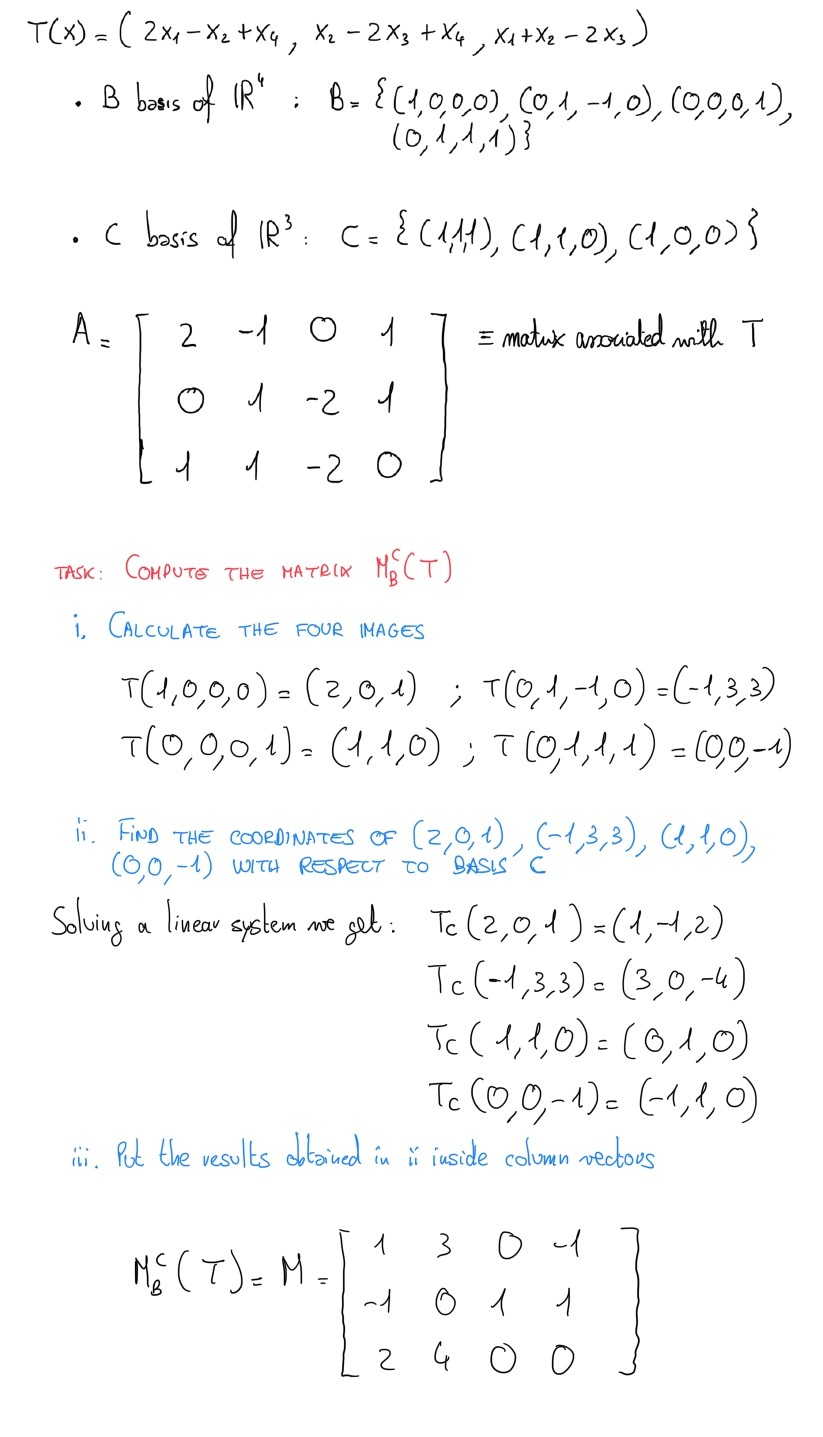
\includegraphics[scale=0.60]{images/04_LinearAlgebra_matrixLinearFunction.jpg}
	\caption{Example of a computation of the matrix associated with a linear
	function}
	\label{fig:linear_function_matrix}
\end{figure}

\defi{\textbf{Matrix of basis transformation} \label{def:basis_transformation}\\ Consider two basis of the vector space $V$: $\mathcal{B}=\{v_{1},...,v_{n}\}$ and $\mathcal{B}'=\{v'_{1},...,v'_{n}\}$. The \textit{transition matrix} (or \textit{matrix of basis transformation}) from $\mathcal{B}$ to $\mathcal{B}'$ is the invertible matrix $P=[p_{ij}]$, with order $n$, whose columns are the coordinates of the vectors $v_{j}$ of the basis $\mathcal{B}$ with respect to the basis $\mathcal{B}'$. \begin{equation*}v_{j}= \sum_{i}p_{ij}v'_{i}\quad (j = 1,...,n)\end{equation*} }

\textbf{Remark:} The matrix $P$ is the matrix associated with the identity
function with respect to the basis $\mathcal{B}$ and $\mathcal{B}'$ :
$P = M^{\mathcal{B}'}_{\mathcal{B}}(id_{V})$. From this observation we can derive
the following consequence. If the vector $v \in V$ has coordinates
$x_{1},...,x_{n}$ with respect to basis $\mathcal{B}$, and coordinates $x'_{1},..
.,x'_{n}$ with respect to basis $\mathcal{B}'$, then:
\begin{equation}
	x' = Px
\end{equation}
where $P$ is the matrix of basis transformation from $\mathcal{B}$ to $\mathcal{B}
'$. We propose an example of basis transformation in $\mathcal{R}^{2}$ in Figure
\ref{fig:basis_transformation}.

\begin{figure}[H]
	\centering
	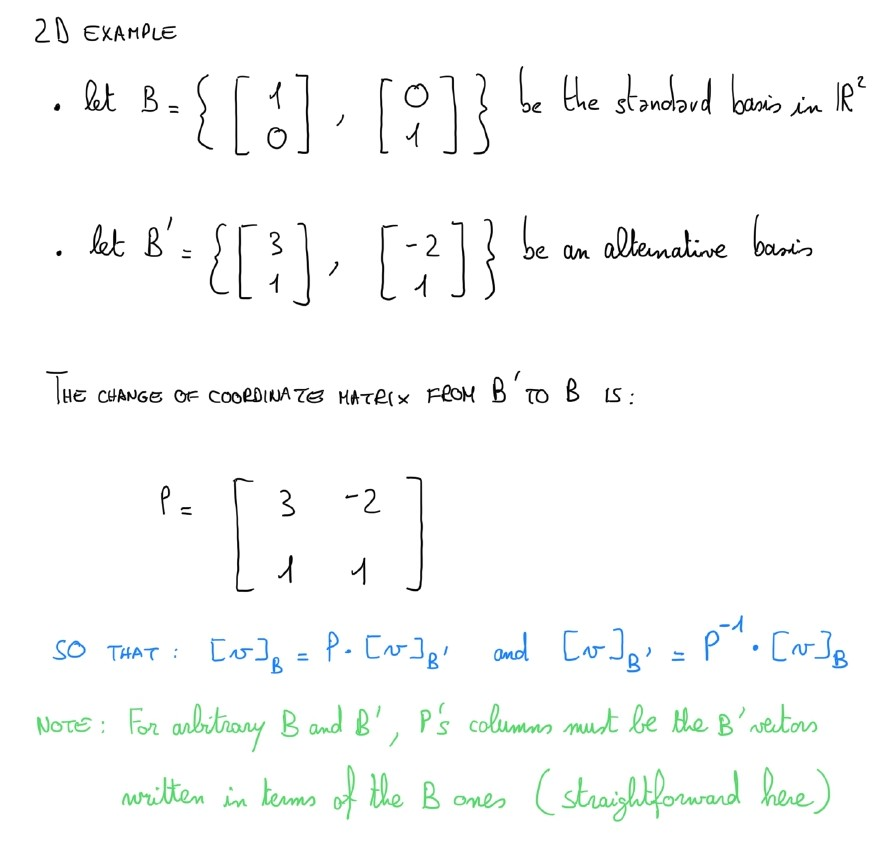
\includegraphics[scale=0.65]{images/04_LinearAlgebra_basisTransformation.jpg}
	\caption{2D example of basis transformation.}
	\label{fig:basis_transformation}
\end{figure}

\defi{\textbf{Transpose} \label{def:transpose}\\ Matrix obtained exchanging rows with columns (indicated with $M^{T}$).\\Given two matrices $M$,$N$ and their transposes $M^{T}$, $N^{T}$, the following relevant property holds: \begin{equation*}(MN)^{T}= N^{T}M^{T}\end{equation*} }

\defi{\textbf{Trace} \label{def:trace}\\ Sum of diagonal elements of a matrix. \begin{equation*}tr(M) = \sum_{i=1}^{n}M_{ii}\end{equation*} }

\defi{\textbf{Inverse} \label{def:inverse}\\ The matrix which multiplied with the original matrix gives the identity. \begin{equation*}MM^{-1}=I\end{equation*} }

\defi{\textbf{Rank} \label{def:rank}\\ The rank of a $n \times m$ matrix is the dimension of the space spanned by its columns. Consider a matrix $A$ $m \times n$. In the matrix there are $n$ columns $A^{1},...,A^{n}$. It is possible to demonstrate that the column space $<A^{1},...,A^{n}>$ has dimension equal to the rank of the matrix $A$. \begin{equation*}rg(A) = \mathit{dim}(<A^{1},...,A^{n}>)\end{equation*} In particular the columns of $A$ are linearly independent if and only if $rg(A)=n$. }

\section{Matrix derivatives}
In this section, there are reported some useful properties of matrix calculus.

\begin{equation*}
	\centering
	\begin{aligned}
		\frac{\partial M \mathbf{x}}{\partial \mathbf{x}}              & =M                                                              \\
		\frac{\partial \mathbf{y}^T M \mathbf{x}}{\partial \mathbf{x}} & =M^{T} \mathbf{y}                                               \\
		\frac{\partial \mathbf{x}^T M \mathbf{x}}{\partial \mathbf{x}} & =\left(M^{T}+M\right) \mathbf{x}                                \\
		\frac{\partial \mathbf{x}^T M \mathbf{x}}{\partial \mathbf{x}} & =2 M \mathbf{x}\quad \text{ if }\mathbf{M}\text{ is symmetric } \\
		\frac{\partial \mathbf{x}^T \mathbf{x}}{\partial \mathbf{x}}   & =2 \mathbf{x}
	\end{aligned}
\end{equation*}

\textbf{Note:} Results are column vectors. Transpose them if row vectors are needed
instead.

\section{Metric structure}
\defi{\textbf{Norm} \label{def:norm}\\ The \textit{norm} defined in $\mathcal{R}^{n}$ is a function $||\cdot||:\mathcal{X}\rightarrow \mathcal{R}_{0}^{+}$ which associates to the vector $x$ the non-negative real number: \begin{equation}||x|| = \sqrt{x \cdot x}= \sqrt{x_{1}^{2}+ ... + x_{n}^{2}}\end{equation} The norm has the following properties: \begin{itemize}\item $||x+y|| \leq ||x|| + ||y||$

\item $||\lambda x|| = |\lambda| ||x||$

\item $||x||>0$ if $x \neq 0$\end{itemize} where $x,y \in \mathcal{X}$, $\lambda \in \mathcal{R}$ }

\defi{\textbf{Metric} \label{def:metric}\\ A norm defines a \textit{metric} $d: \mathcal{X}\times \mathcal{X}\rightarrow \mathcal{R}_{0}^{+}$ such that: \begin{equation}d(x,y) = ||x-y||\end{equation} This metric is commonly referred to as $distance$. This latter is a function which associates to each couple of vectors $x,y \in \mathcal{R}^{n}$ the real number $d(x,y)$. }

\textbf{Remark:} The concept of norm is stronger than that of metric: not any metric
gives rise to a norm.\\

\defi{\textbf{Unit vector} \label{def:unit_vector}\\ A \textit{unit vector} is a vector $v \in \mathcal{R}^{n}$ such that: \begin{equation*}||v|| = 1\end{equation*} }

\textbf{Remark:} each vector $v \neq \pmb{0}$ can be normalized:
\begin{equation*}
	v' = \frac{v}{||v||}
\end{equation*}
where $v'$ is a unit vector.

\section{Dot product}
\defi{\textbf{Bilinear form} \label{def:bilinear_form}\\ A function $Q: \mathcal{X}\times \mathcal{X}\rightarrow \mathcal{R}$ on a vector space $X$ is a \textit{bilinear form} if it is linear in each argument separately: \begin{equation*}Q(\lambda x + \mu y, z) = \lambda Q(x,z) + \mu Q(y,z)\end{equation*}

\begin{equation*}Q(x, \lambda y + \mu z) = \lambda Q(x,y) + \mu Q(x,z)\end{equation*} where $x,y,z \in \mathcal{X}$, $\lambda, \mu \in \mathcal{R}$.

A bilinear form is \textit{symmetric} if for all $x,y \in \mathcal{X}$: \begin{equation*}Q(x,y) = Q(y,x)\end{equation*}

}

\defi{\textbf{Dot product} \label{def:dot_product}\\ The \textit{dot product} on $\mathcal{R}^{n}$ is a function $<\cdot,\cdot>: \mathcal{X}\times \mathcal{X}\rightarrow \mathcal{R}$ which associate to a couple of vectors $x,y \in \mathcal{R}^{n}$ the real number: \begin{equation}<x,y> = x \cdot y = \sum_{i=1}^{n}x_{i}y_{i}= x^{T}y\end{equation} }

The dot product has the following properties:
\begin{enumerate}
	\item \textit{symmetric}: $x \cdot y = y \cdot x$ for all $x,y \in \mathcal{R}^{n}$

	\item \textit{bilinear}: $(\alpha x + \beta y) \cdot z = \alpha (x \cdot z) + \beta
		(y \cdot z)$ and $x \cdot (\alpha y + \beta z) = \alpha (x \cdot y) + \beta (
		x \cdot z)$, for all $x,y,z \in \mathcal{R}^{n}$ and
		$\alpha, \beta \in \mathcal{R}$

	\item \textit{symmetric bilinear}: this property follows from the previous ones

	\item \textit{positive semi-definite}: $x \cdot x \geq 0$ for all $x \in \mathcal{R}
		^{n}$

	\item The dot product could also be \textit{positive definite} if it satisfies:
		$x \cdot x = 0$ iff $x=0$ for all $x \in \mathcal{R}^{n}$
\end{enumerate}

Any dot product defines a corresponding \textit{norm} via:
\begin{equation*}
	||x|| = \sqrt{<x,x>}
\end{equation*}

\begin{itemize}
	\item The angle $\theta$ between two vectors is defined as:
\end{itemize}
\begin{equation}
	\cos{\theta}= \frac{<x,z>}{||x||||z||}
\end{equation}

\begin{itemize}
	\item Two vectors are \textit{orthogonal} if $<x,y>=0$.

	\item A set of vectors $\{x_{1},...,x_{n}\}$ is orthonormal if all vectors $x_{i}$
		in the set are mutually orthogonal and are all unit vectors:
\end{itemize}
\begin{equation*}
	<x_{i}, x_{j}> = \delta_{ij}
\end{equation*}
\hspace{7mm} where $\delta_{ij}=1$ if $i=j$, $0$ otherwise.

\section{Eigenvalues and eigenvectors}
\label{sec:eigenvalues_eigenvectors}

\defi{\textbf{Eigenvalues and eigenvectors} \label{def:eigen}\\ Given a $n \times n$ matrix $M$, the real value $\lambda$ and (non-zero) vector $x$ are an \textit{eigenvalue} and corresponding \textit{eigenvector} of $M$ if: \begin{equation}Mx=\lambda x\end{equation} }

\textbf{Properties:}
\begin{itemize}
	\item A $n \times n$ matrix has $n$ eigenvalues

	\item A $n \times n$ matrix can have less than $n$ distinct eigenvalues

	\item A $n \times n$ matrix can have less than $n$ linear independent eigenvectors
		(also fewer then the number of distinct eigenvalues)
\end{itemize}

\defi{\textbf{Singular matrices} \label{def:singular_matrix}\\ A matrix is \textit{singular} if it has a zero eigenvalue. \begin{equation*}Mx = 0x = 0\end{equation*} }

A singular matrix has linearly dependent columns (see Definition \ref{def:indipendency1}):
\begin{equation*}
	[M_{1}... M_{n-1}M_{n}]
	\begin{bmatrix}
		x_{1}   \\
		x_{2}   \\
		\vdots  \\
		x_{n-1} \\
		x_{n}
	\end{bmatrix}
	= 0
\end{equation*}
\begin{equation*}
	M_{1}x_{1}+\hdots+M_{n-1}x_{n-1}+M_{n}x_{n}= 0
\end{equation*}
\begin{equation*}
	M_{n}= M_{1}\frac{-x_{1}}{x_{n}}+\hdots+M_{n-1}\frac{-x_{n-1}}{x_{n}}
\end{equation*}

\defi{\textbf{Determinant} \label{def:determinant}\\ The \textit{determinant} $|M|$ of a $n \times n$ matrix $M$ is the product of its eigenvalues. }

\textbf{Remark:} a matrix is \textit{invertible} if its determinant is not zero
(i.e. it is not singular).

\defi{\textbf{Symmetric matrix} \label{def:symmetric_matrix}\\ A \textit{symmetric matrix} is a square matrix that is equal to its transpose. \begin{equation*}A = A^{T}\end{equation*} Because equal matrices have equal dimensions, only square matrices can be symmetric. The entries of a symmetric matrix are symmetric with respect to the main diagonal. So if $a_{ij}$ denotes the entry in the $i$th row and $j$th column then: \begin{equation*}a_{ji}= a_{ij}\end{equation*} for all indices $i$ and $j$. }

If A is a real symmetric matrix, then any two eigenvectors ($x,z$) corresponding
to distinct eigenvalues ($\lambda \neq \mu$) are orthogonal. $(x, \lambda)$ and $(
z, \mu)$ IF $\lambda \neq \mu \Rightarrow <x,z>=0$. The proof of this
preposition is reported in Figure \ref{fig:proof_eigen_symmetric}.

\begin{figure}[H]
	\centering
	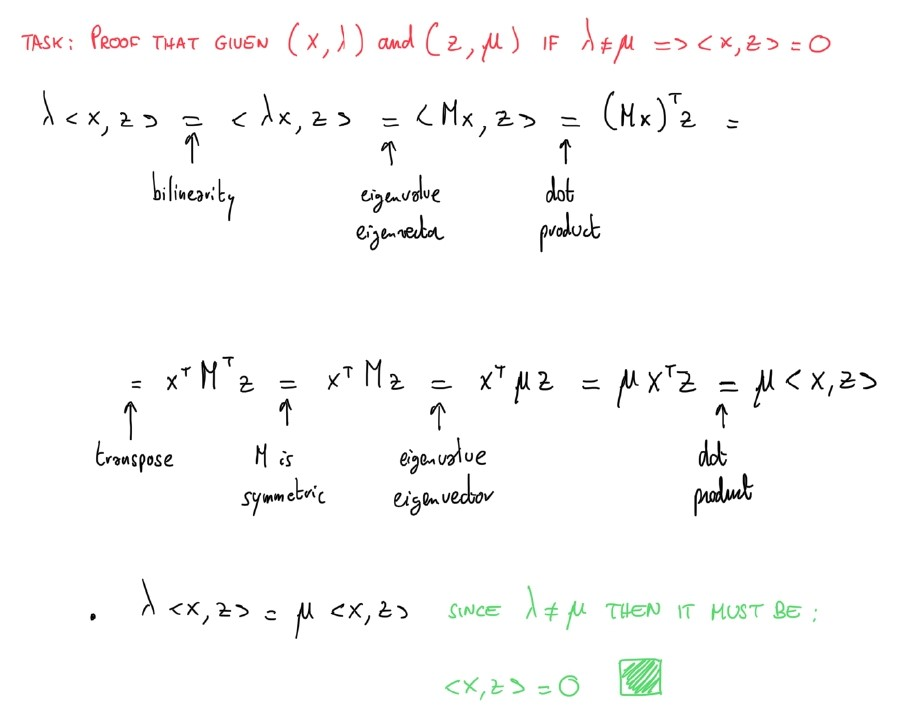
\includegraphics[scale=0.85]{images/04_LinearAlgebra_symmetricMatrixProof.jpg}
	\caption{Proof that $(x, \lambda)$ and $(z, \mu)$ IF
	$\lambda \neq \mu \Rightarrow <x,z>=0$.}
	\label{fig:proof_eigen_symmetric}
\end{figure}

\section{Eigen-decomposition}
The purpose of this section is to describe an iterative procedure to find eigenvalues
and eigenvectors for a matrix $A$. Given $A$ we want to find $\lambda$ and $x$
values such that:

\begin{equation*}
	Ax=\lambda x
\end{equation*}

We multiply both sides of the equation by $x^{T}$ and we divide both sides of the
equation by $x^{T}x$. We are not interested in the 0 vector, so the dot product $x
^{T}x$ is not 0.

\begin{equation*}
	\frac{x^{T}A x}{x^{T}x}= \frac{x^{T}\lambda x}{x^{T}x}
\end{equation*}

For linearity we can move $\lambda$.

\begin{equation*}
	\frac{x^{T}A x}{x^{T}x}= \lambda \frac{x^{T}x}{x^{T}x}= \lambda
\end{equation*}

The fraction $\frac{x^{T}A x}{x^{T}x}$ is called \textit{Raleigh quotient}.

\paragraph{}

At this point we want to find the eigenvector which maximize the \textit{Raleigh
quotient}. In this way we get the eigenvector ($x$) which corresponds to the maximal
eigenvalue.

\begin{equation*}
	x = \mathit{argmax}_{v}\frac{v^{T}A v}{v^{T}v}
\end{equation*}

Now we normalize the obtained eigenvector $x$:
\begin{equation*}
	x \leftarrow \frac{x}{||x||}
\end{equation*}

Note that a normalized eigenvector is still an eigenvector.

In this way we have obtained the first eigenvalue and the first normalized
eigenvector.

\paragraph{}

In order to compute the other eigenvectors and eigenvalues, we modify $A$ such that,
if we repeat the previous procedure, we find another eigenvector. This
modification is called \textit{deflation}.

\begin{equation*}
	\tilde{A}= A - \lambda x x^{T}
\end{equation*}

Note that $x x^{T}$ is not $x^{T}x$ which is a scalar (dot product). Indeed $x x^{T}$
is a matrix.

Deflation turns $x$ into an eigenvector for $\tilde{A}$ which has zero-eigenvalue:

\begin{equation*}
	\tilde{A}x = (A - \lambda x x^{T}) x = Ax - \lambda x x^{T}x
\end{equation*}
Since $x$ is normalized $x^{T}x = 1$, so:
\begin{equation*}
	\tilde{A}x = Ax - \lambda x
\end{equation*}
Since $\lambda$ and $x$ is an eigenvalue-eigenvector pair $Ax = \lambda x$, so:
\begin{equation*}
	\tilde{A}x = Ax - \lambda x = 0
\end{equation*}
We can conclude that $x$ is an eigenvector with 0 eigenvalue:
\begin{equation*}
	\tilde{A}x = 0x
\end{equation*}

\paragraph{}
At this point, we can repeat the maximization procedure on the deflated matrix.
In particular, we maximize the Raleigh quotient $\frac{v^{T}\tilde{A}v}{v^{T}v}$.
In this way we can find the maximal possible eigenvalue. For sure, we will not
find $x$ since its corresponding eigenvalue is 0. We can demonstrate that after
the deflation operation, other eigenvalues-eigenvectors are unchanged:
\begin{equation*}
	\tilde{A}z = (A - \lambda x x^{T}) z = Az - \lambda x x^{T}z
\end{equation*}
As stated in Section \ref{sec:eigenvalues_eigenvectors}, in the case of symmetric
matrices, eigenvectors with distinct eigenvalues are orthogonal, so:
\begin{equation*}
	\tilde{A}z = Az - \lambda x x^{T}z = Az
\end{equation*}
As a conclusion, for a symmetric matrix, dealing with $\tilde{A}$ is like
working with $A$.

\paragraph{}
At the end of the day:
\begin{equation*}
	x' = \textit{argmax}_{v}\frac{v^{T}\tilde{A}v}{v^{T}v}
\end{equation*}
where $x'$ is the eigenvector with the second largest eigenvalue. The procedure is
iteratively repeated on the deflated matrix until solution is zero, which means
that there are no more positive eigenvalues. If the matrix has negative eigenvalues,
I can recover them minimizing the Raleigh quotient instead of maximizing it. At some
point the solution of the iterative procedure will be 0 again. If the obtained
set of eigenvalues is not full rank yet, we have to take into consideration the eigenvectors
with zero eigenvalues. The eigenvectors with zero eigenvalues are obtained
extending the obtained set to an orthonormal basis.

\paragraph{}
Eigen-decomposition allows to diagonalize a matrix.

\begin{itemize}
	\item Let $V = [v_{1}\hdots v_{n}]$ be a matrix with orthonormal eigenvectors as
		columns

	\item Let $\Lambda$ be the diagonal matrix of corresponding eigenvalues

	\item A square simmetric matrix can be \textit{diagonalized} as:
\end{itemize}
\begin{equation}
	V^{T}A V = \Lambda
\end{equation}

\textbf{Remark:} a diagonalized matrix is much simpler to manage and has the same
properties as the original one (e.g. same eigen-decomposition).

\vspace{5mm}

\textbf{Proof:}\\ From eigenvalue-eigenvector definition (Definition
\ref{def:eigen}):
\begin{equation*}
	A[v_{1}\hdots v_{n}] = [v_{1}\hdots v_{n}]
	\begin{bmatrix}
		\lambda_{1} &        & 0           \\
		            & \ddots &             \\
		0           &        & \lambda_{n}
	\end{bmatrix}
\end{equation*}
\begin{equation*}
	AV = V \Lambda
\end{equation*}

We multiply both sides by $V^{-1}$.
\begin{equation*}
	V^{-1}AV = V^{-1}V \Lambda
\end{equation*}

We have that $V^{-1}V = I$. What is more $V$ is a \textit{unitary matrix}, which
means that its columns are orthonormal, for which: $V^{-1}= V^{T}$. As a consequence:
\begin{equation*}
	V^{T}AV = \Lambda
\end{equation*}

\defi{\textbf{Positive semi-definite matrix} \label{def:positive_semidefinite_matrix}\\ An $n \times n$ symmetric matrix $M$ is \textit{positive semi-definite} if all its eigenvalues are non-negative. Alternative sufficient and necessary conditions are: \begin{itemize}\item for all $x \in \mathcal{R}^{n}$\end{itemize} \begin{equation*}x^{T}M x \geq 0\end{equation*} \begin{itemize}\item there exists a real matrix $B$ such that:\end{itemize} \begin{equation*}M = B^{T}B\end{equation*} }

\defi{\textbf{Positive definite matrix} \label{def:positive_definite_matrix}\\ An $n \times n$ symmetric matrix $M$ is \textit{positive definite} if all its eigenvalues are positive. }

\section{Understanding eigendecomposition}

\subsection{Scaling transformation in standard basis}
Consider Figure \ref{fig:scalar_trans}.
\begin{itemize}
	\item Let $x_{1}= [1,0]$, $x_{2}= [0,1]$ be the standard orthonormal basis in
		$\mathcal{R}^{2}$

	\item Let $x = [x_{1}, x_{2}]$ be an arbitrary vector in $\mathcal{R}^{2}$

	\item A linear transformation is a \textit{scaling} transformation if it only
		stretches $x$ along its directions
\end{itemize}

In Figure \ref{fig:scalar_trans}, matrix $A$ encodes a scaling transformation.

\begin{figure}[H]
	\centering
	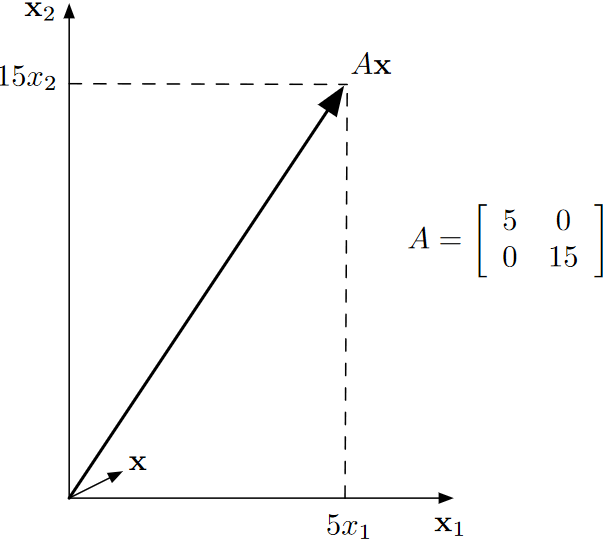
\includegraphics[width=0.5\textwidth]{
		images/04_LinearAlgebra_scalingVector.png
	}
	\caption{Scaling transformation in standard basis.}
	\label{fig:scalar_trans}
\end{figure}

\subsection{Scaling transformation in eigenbasis}
Consider Figure \ref{fig:eigenbasis_trans}.
\begin{itemize}
	\item Let $A$ be a non-scaling linear transformation in $\mathcal{R}^{2}$.
		Actually, transformation $Av$ is not a linear transformation, since $v$ has
		no components along the x\-axis.

	\item Let $\{v_{1}, v_{2}\}$ be an \textit{eigenbasis} for $A$. An eigenbasis is
		a basis in which every vector is an eigenvector.

	\item By representing vectors in $\mathcal{R}^{2}$ in terms of the $\{v_{1},v_{2}
		\}$ basis (instead of the standard $\{x_{1}, x_{2}\}$), $A$ becomes a
		scaling transformation.
\end{itemize}

Eigendecomposition is useful since we can compute an eigenbasis for a matrix $A$
so that $A$ becomes a scaling transformation with respect to the coordinate
system defined by the eigenbasis.

\begin{figure}[H]
	\centering
	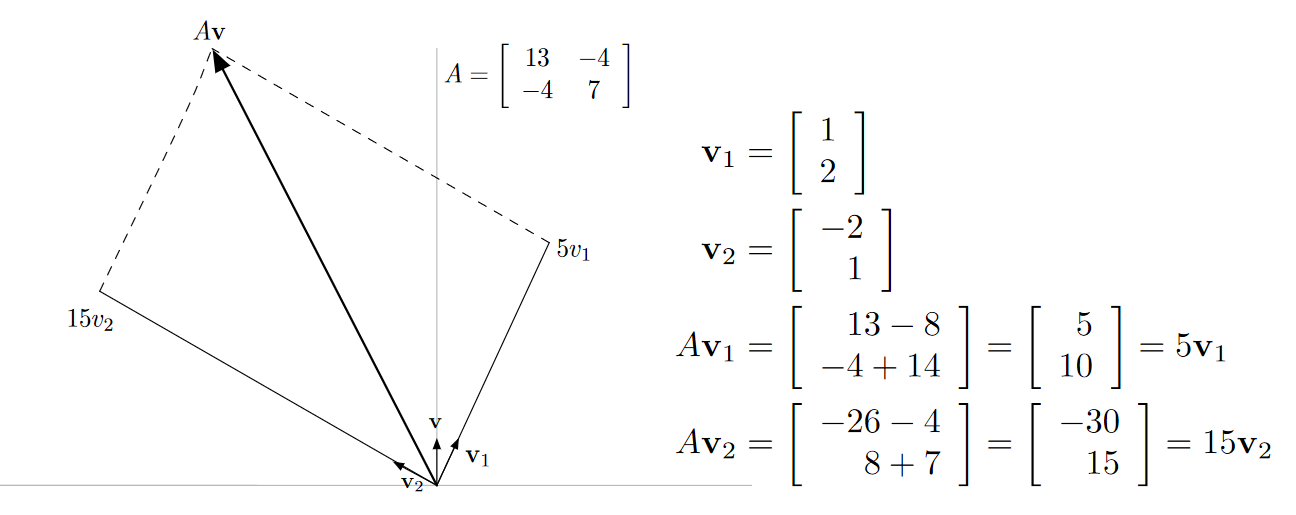
\includegraphics[width=\textwidth]{
		images/04_LinearAlgebra_eigenbasisTransformation.png
	}
	\caption{Scaling transformation in eigenbasis.}
	\label{fig:eigenbasis_trans}
\end{figure}

\section{Principal Component Analysis (PCA)}
Consider Figure \ref{fig:eigen_PCA}. $X$,$Y$ could be the height and the weight
of a person. These two dimensions are correlated. As a result, if we collect some
data from a population, we would obtain a distribution similar to the one
represented on the left side of Figure \ref{fig:eigen_PCA}. On the other hand,
the graphic on the right of Figure \ref{fig:eigen_PCA}, represents two quantities
$P1, P2$ which are apparently uncorrelated. Indeed, the data spreads along the two
dimensions.

\begin{itemize}
	\item Let $A$ be a data matrix with correlated coordinates.

	\item PCA is a linear transformation mapping data to a system of uncorrelated coordinates.

	\item It corresponds to fitting an ellipsoid to the data, whose axes are the
		coordinates of the new space.
\end{itemize}

\begin{figure}[H]
	\centering
	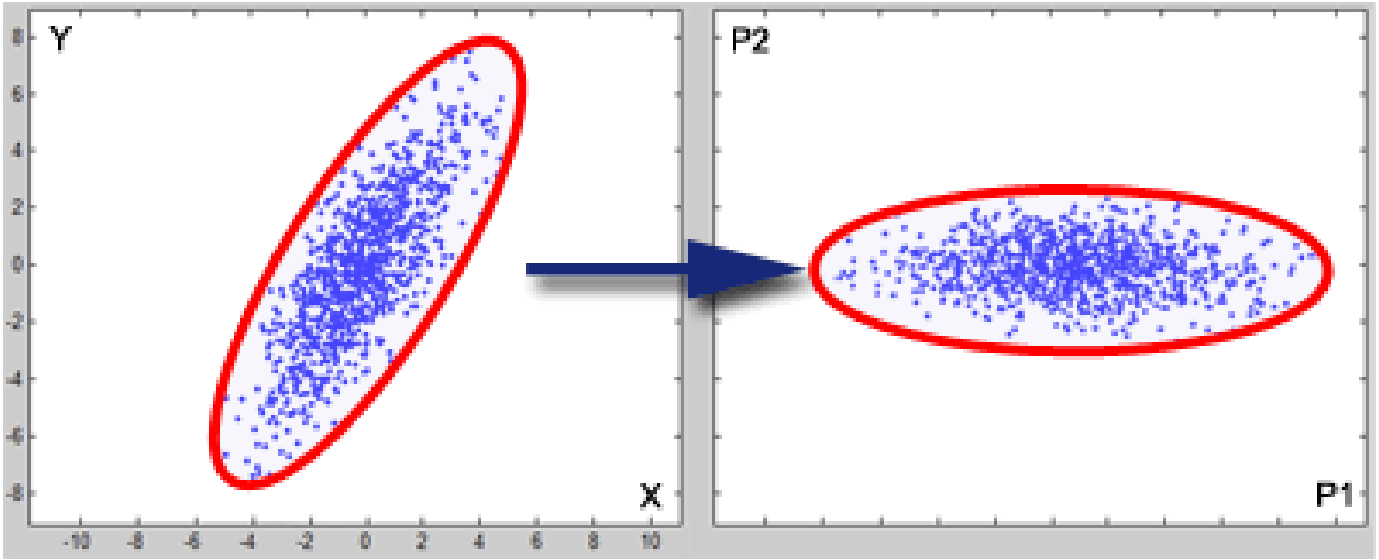
\includegraphics[width=\textwidth]{images/04_LinearAlgebra_PCA.png}
	\caption{Principal Component Analysis (PCA).}
	\label{fig:eigen_PCA}
\end{figure}

Given a dataset $X \in \mathcal{R}^{n \times d}$ with $n$ examples and $d$ dimensions.

\begin{enumerate}
	\item Compute the mean of the data ($X_{i}$ is the $i^{th}$ row vector of $X$):
		\begin{equation*}
			\Bar{x}= \frac{1}{n}\sum_{i=1}^{n}X_{i}
		\end{equation*}

	\item Center the data into the origin:
		\begin{equation*}
			X = X -
			\begin{bmatrix}
				\Bar{x} \\
				\vdots  \\
				\Bar{x}
			\end{bmatrix}
		\end{equation*}

	\item Compute the data covariance:
		\begin{equation*}
			C = \frac{1}{n}X^{T}X
		\end{equation*}
		The covariance information highlights the correlations between the
		dimensions.

	\item Compute the (orthonormal) eigendecomposition of $C$:
		\begin{equation*}
			V^{T}C V = \Lambda
		\end{equation*}

	\item Use the set of eigen vectors as the new coordinate system:
		\begin{equation*}
			x' = V^{-1}x = V^{T}x
		\end{equation*}
		($V^{-1}= V^{T}$ as $V$ is unitary). In this new space (represented by the
		axis of the ellipse) the data are uncorrelated.
\end{enumerate}

\textbf{Remark:} this procedure assumes linear correlations (and Gaussian
distributions).

\subsection{Dimensionality reduction}
Assume that we have computed the covariance matrix $C$ of a certain data distribution.
What is more, we have also performed eigen value - eigen vector decomposition.
At this point, it is possible to proof that each eigenvalue corresponds to the amount
of variance in the direction of the corresponding eigenvector. The eigen vector
which corresponds to the largest eigen values represents the directions of
largest spread. The dimensions with the largest spread are the dimensions with the
largest information. In order to perform \textit{dimensionality reduction} (e.g.
visualization), we select only the $k$ eigenvectors with largest eigenvalues.\\ Suppose
that we want to map the data in a $d$ dimensional space in a lower dimensional space
with $k$ dimensions. To do this, we execute the same procedure described above for
PCA, but this time we take into consideration only the first $k$ eigenvectors of
the covariance matrix decomposition.
\begin{equation*}
	W = [v_{1}, \hdots, v_{k}]
\end{equation*}
Then, it is straightforward to map a point in the primary space to the new lower
$k$-dimensional space (which retains the most information in terms of linear correlations):
\begin{equation*}
	x' = W^{T}x
\end{equation*}

Dimensionality reduction could be a valid pre-computation before applying other
machine learning algorithms which perhaps performs poorly on high dimensional
scenarios.